%!TEX root = ../proteoform_suite_manual.tex
%---------------------------------------------------------------------
%	NEUCODE PAIRS
%---------------------------------------------------------------------

\section{NeuCode Pairs}

\subsection{Overview}

On this page, NeuCode pairs are generated from the raw experimental components. Each NeuCode pair consists of a light raw experimental component and a heavy raw experimental component; the lysine count is determined based upon the delta mass difference between the light and heavy raw experimental components of the NeuCode pair. For more information on generating NeuCode labeled data for proteoform identification in Proteoform Suite, see the methods sections of previously published analyses.\supercite{Shortreed2016,Cesnik2018,Dai2017,Dai2019} 

\subsection{Run Page}
\begin{itemize}
\item The Raw Experimental Components page must be run before running this page
\item Click Run Page button (top right)
\item Set all parameters as desired for current analysis (see below). The results automatically refresh; you do not need to re-run the page after adjusting the parameters. Only accepted NeuCode pairs will be included in further analysis in Proteoform Suite.
\end{itemize}

\subsection{Set Parameters}
\begin{figure}[h]
\centering
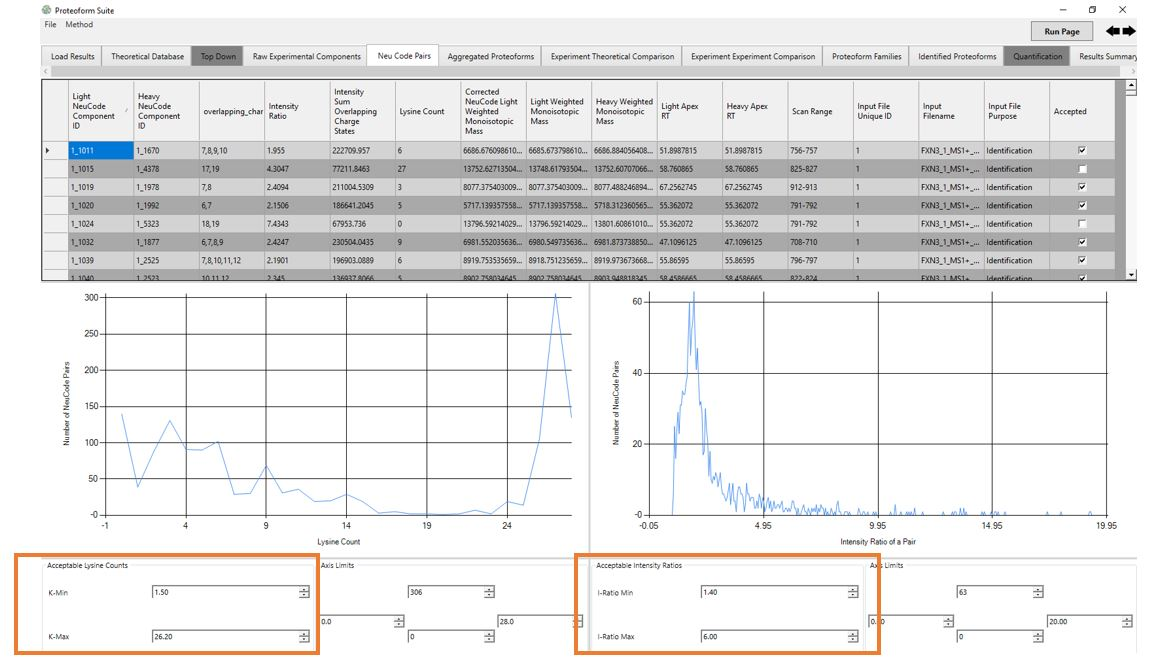
\includegraphics[scale=0.43]{figures/neucode1.jpg}
\end{figure}
\begin{itemize}
\item Acceptable Lysine Counts: only NeuCode pairs with an acceptable number of lysines will be accepted
\begin{itemize}
\item K-Min: minimum acceptable lysine count for a NeuCode pair to be accepted for further analysis
\item K-Max: maximum acceptable lysine count for a NeuCode pair to be accepted for further analysis
\end{itemize}
\item Acceptable Intensity Ratios: only NeuCode pairs with an acceptable intensity ratio between light/heavy raw experimental components will be accepted
\begin{itemize}
\item I-Ratio Min: minimum acceptable intensity ratio for a NeuCode pair to be accepted for further analysis
\item I-Ratio Max: maximum acceptable intensity ratio for a NeuCode pair to be accepted for further analysis
\end{itemize}
\end{itemize}

\subsection{Results}
\begin{itemize}
	\item NeuCode pairs table: the top table displays all NeuCode pairs generated
	\begin{figure}[h]
\centering
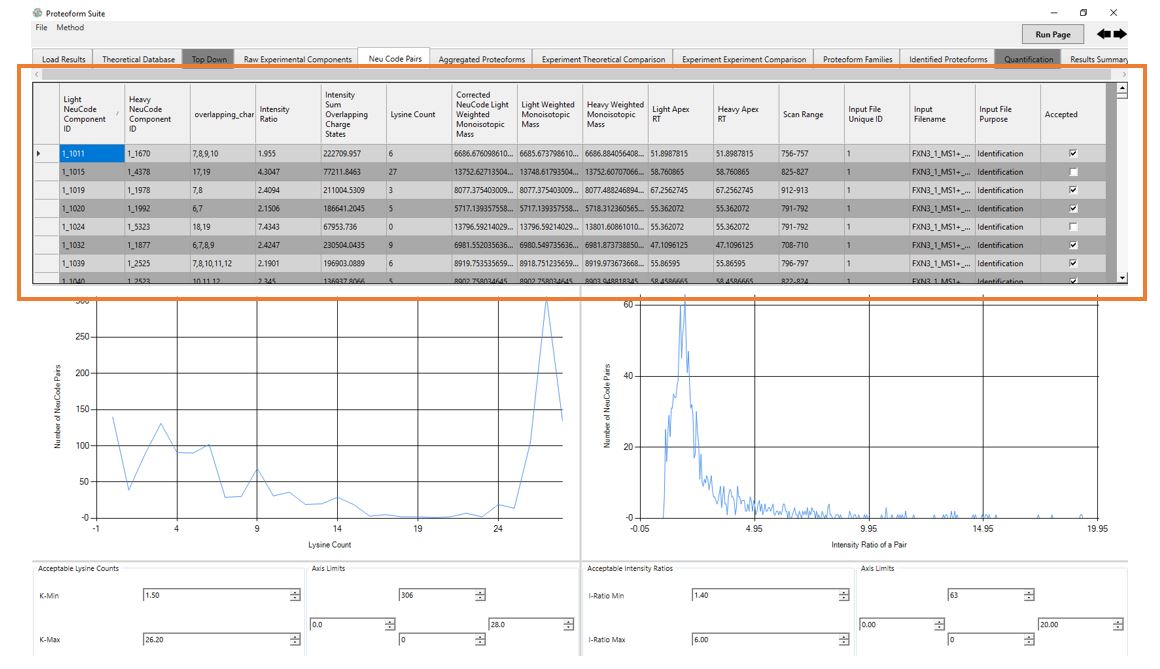
\includegraphics[scale=0.5]{figures/neucode2.jpg}
\end{figure}
\begin{itemize}
		\item Light NeuCode Component ID: Proteoform Suite given ID for the light raw experimental component; file ID\_component \#
		\item Heavy NeuCode Component ID: Proteoform Suite given ID for the heavy raw experimental component; file ID\_component \#
		\item Overlapping Charge States: comma-separated list of charge states observed for both the light and heavy raw experimental components components in this NeuCode pair
		\item Intensity Ratio: intensity ratio of light raw experimental component intensity : heavy raw experimental component intensity
		\item Intensity Sum Overlapping Charge States: summed intensity for all charge states observed for both the light and heavy raw experimental components in this NeuCode pair
		\item Lysine Count: lysine count for this NeuCode pair; determined by mass difference between light and heavy raw experimental components
		\item Corrected NeuCode Light Weighted Monoisotopic Mass: monoisotopic mass of light raw experimental component used for this NeuCode pair, monoisotopic mass errors corrected
		\item Light Weighted Monoisotopic Mass: monoisotopic mass of light raw experimental component
		\item Heavy Weighted Monoisotopic Mass: monoisotopic mass of heavy raw experimental component
		\item Light Apex RT: apex retention time of light raw experimental component
		\item Scan Range: MS scan range for light and heavy raw experimental components in this NeuCode pair
		\item Input File Unique ID: file ID number for filename of Deconvolution Results for Identification or Quantification for the light and heavy raw experimental components in this NeuCode pair
		\item Input Filename: filename of Deconvolution Results for Identification or Quantification for light and heavy raw experimental components in this NeuCode pair
		\item Input File Purpose: either Identification or Quantification
		\item Accepted: checked if this NeuCode pair has a lysine count and intensity ratio within the min and max range allowed (see Set Parameters); if accepted, this NeuCode pair will be utilized in subsequent Proteoform Suite analysis
\end{itemize}
\item Lysine Count histogram: the left graph shows a histogram of lysine counts for all NeuCode pairs. The Axis Limits box below this graph adjusts the x- and y-axes.
	\begin{figure}[h]
\centering
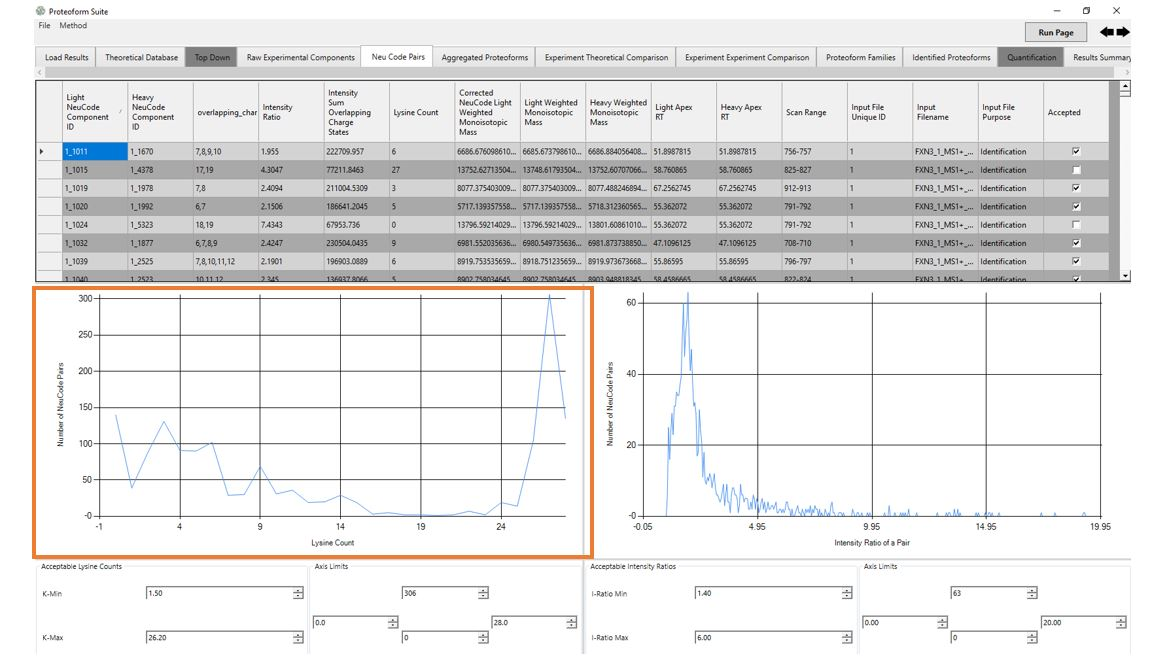
\includegraphics[scale=0.5]{figures/neucode3.jpg}
\end{figure}
\pagebreak
\item Intensity Ratio histogram: the right graph shows a histogram of light:heavy intensity ratios for all NeuCode pairs. The peak of this histogram should fall close to the experimentally performed mixing ratio for light:heavy protein samples (ex: 2:1 light:heavy). The Axis Limits box below this graph adjusts the x- and y-axes.
	\begin{figure}[h]
\centering
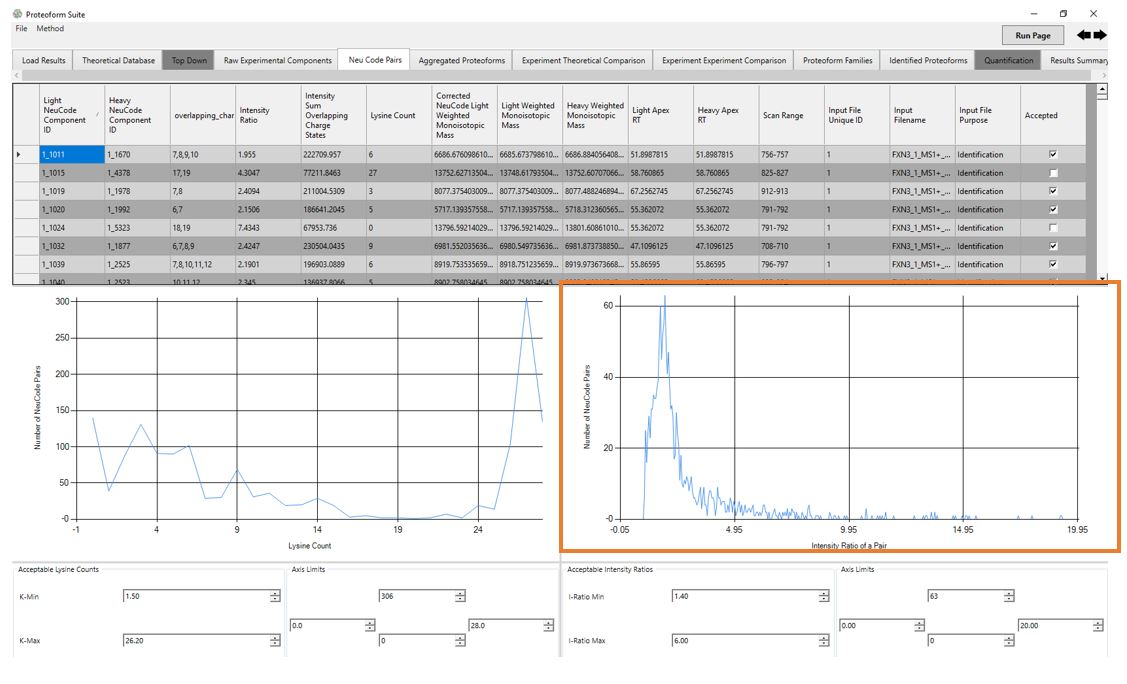
\includegraphics[scale=0.5]{figures/neucode4.jpg}
\end{figure}
\end{itemize}